
\section{Methodology} \label{sec:method}

To address the identified gaps and support the goal of designing efficient, reliable, and safe LT-PEMFC systems for aircraft, we propose a modelling and methodological framework to enable detailed and efficient exploration of optimal aircraft and power system design. This proposed system will incorporate:
\begin{enumerate}
	\item Multi-scale and multi-physics LT-PEM cell models.
	\item Parametric stack, TMS, WMS, fuel supply, and air supply models.
	\item Advanced physics-aware multi-fidelity surrogate models.
	\item A computational framework for dynamic fuel cell system modeling.
	\item Advanced computational methods to efficiently explore optimal system design.
\end{enumerate}
The following subsection will outline the models and methods that comprise the proposed framework.

\subsection{Cell \& Stack Modelling}
High-fidelity fuel cell models are commonly posed as sets of coupled partial differential equations (PDEs) expressing conservation laws for mass, momentum, species, charge, and energy.
Domains within the cell such as the channel, GDL, catalyst, and membrane are differentiated by their source terms. The resulting PDEs are solved over a discretised domain using either Finite Element Methods (FEMs) or Finite Volume Methods (FVMs).
FEMs offer simplified treatment of higher coupling, simpler incorporation of complex geometries, and easier adaptation to higher order methods, whilst FVMs ensure strict adherence to the conservation laws.
There has been a longstanding reluctance in the fuel cell modelling comunity to open source their fuel cell models.
This has changed in the last few years with a growing number of open source models being released and maintained \cite{vetterFreeOpenReference2019, secanellOpenFCSTOpenSourceMathematical2014, zhangOpenFuelCell2NewComputational2024,  koneOpenSourceToolboxPEM2018, gassAlphaPEMOpensourceDynamic2025}.
This has been fuelled by continued improvements in conventional and parallel computing hardware.
We aim to use these open source models to build a set of parametric LT-PEM cell and stacks.
Detailed thermal and hydration effects will capture through computationally expensive multi-physics models \cite{secanellOpenFCSTOpenSourceMathematical2014, zhangOpenFuelCell2NewComputational2024, vetterFreeOpenReference2019}, whilst scaling effects will be captured through models considering higher spatial dimensions \cite{secanellOpenFCSTOpenSourceMathematical2014, zhangOpenFuelCell2NewComputational2024, koneOpenSourceToolboxPEM2018}.
Lower-fidelity models will supplement by enabling efficient exploration of the design space \cite{kulikovskyPhysicallyBasedAnalytical2013a, ohayreFuelCellFundamentals2016, larminieFuelCellSystems2003}. In the following section we will outline the lowest and highest fidelity models we intend to use.

\subsubsection{Low Fidelity Model}

We propose the use of a semi-empirical quasi-one-dimensional model presented by Kulikovsky \cite{kulikovskyPhysicallyBasedAnalytical2013a}.
The cell model comprises approximate solutions to a generalised one-dimensional cathode catalyst layer model under different limiting assumptions.
\begin{equation}
	\frac{\diff \wt{j}}{\diff \wt{x}}      = -\frac{\wt{c}}{\varepsilon}\sinh{\wt{\eta}}, \quad
	\frac{\diff \wt{\eta}}{\diff \wt{x}}  = -\wt{j}, \quad
	\frac{\diff \wt{c}}{\diff \wt{x}}      = \frac{1}{\wt{D}}\left(\wt{j}_0 - \wt{j}\right)
\end{equation}
Note that nondimensional quantities are marked with a tilde. Specifically, for a scalar value \( x \in \mathbb{R} \), we define the corresponding non-dimensional value as
\[
	\wt{x} = \mathcal{S}(x),
\]
where \( \mathcal{S} \) denotes a general non-dimensionalisation map that scales \( x \) by appropriate reference quantities. The inverse map is denoted \( \mathcal{S}^{-1} \), so that
\[
	x = \mathcal{S}^{-1}(\wt{x}).
\]

Assuming ideal oxygen transport, that is to say diffusivity $D \rightarrow \infty$, Kulikovsky derived an expression for the combined oxygen reduction reaction activation and proton transport overpotentials as a function of the proton current density $j_0$, where $\varepsilon$ is Newman's dimensionless reaction penetration depth, and $c_1$ is the oxygen concentration at the interface of the CCL and GDL.
\begin{equation}
	\arcsinh{\frac{\varepsilon^2 \wt{j}_0^2}{2 \wt{c}_1 \left(1 - \exp{\frac{-\wt{j}_0}{2}}\right)}} \label{eq:eta}
\end{equation}
Order reduction techniques and an assumption of high current density allow the derivation of the following approximation to the oxygen transport overpotential.
\begin{equation}
	\frac{1}{\wt{D}\wt{c}_1}\left(\wt{j}_0 - \ln\left(1 + \frac{\wt{j}_0^2}{\beta^2}\right)\right) \label{eq:etad}
\end{equation}
Where $\beta$ is the approximate solution to
\begin{equation}
	\beta \tan{\frac{\beta}{2}} = \wt{j}_0, \quad 0 \le \beta < \pi
\end{equation}
An assumption of constant oxygen concentration gradient in the GDL enabled a substitution of equation \ref{eq:oxyconc} equation \ref{eq:etad} to reframe the problem in terms of the oxygen concentration in the channel $c_h$ and limiting current density due to oxygen transport in the GDL $j_{\text{lim}}$. The Tafel law was used to account for oxygen transport losses in the GDL, yielding the final GDL, and CCL overpotential model igen in equation \ref{eq:kulfull}.

\begin{equation}
	\wt{c}_1 = \wt{c}_h \left(1 - \frac{\wt{j}_0}{\wt{j}_{\text{lim}}\wt{c}_h}\right)\label{eq:oxyconc}
\end{equation}

\begin{equation}
	\wt{\eta}_0(\wt{j}_0) = \arcsinh{\frac{\varepsilon^2 \wt{j}_0^2}{2 \wt{c}_1 (1 - \exp{\frac{-\wt{j}_0}{2}})}}
	+ \frac{1}{\wt{D}\wt{c}_h}\left(\wt{j}_0 - \ln\left(1 + \frac{\wt{j}_0^2}{\beta^2}\right)\right)\left(1 - \frac{\wt{j}_0}{\wt{j}_{\text{lim}}\wt{c}_h}\right)^{-1}
	-\left(1 - \frac{\wt{j}_0}{\wt{j}_{\text{lim}}\wt{c}_h}\right)
	\label{eq:kulfull}
\end{equation}

The cell polarisation curve may then be estimated using the open-circuit potential $E$, and the cell resistance \(R_{\Omega}\).
\begin{equation}
	V(i) = E - \eta_0(i) - iR_\Omega
\end{equation}

The computational cost of this model is negligible compared to FEM and FVM approaches whilst providing a physicaly based solution. For these reasons it is well suited to be provide the lowest fidelity solution for the proposed surrogate model.

\subsubsection{High Fidelity Model}

\subsection{Surrogate Modelling}
We propose the use of the surrogate and active learning method to learn a latent representation of the stack current density $i$ as a function of open-circuit normalised mean cell voltage $v$ and system design parameters $\bm{x}_0, \bm{x}_{\text{BoP}}, \bm{x}_{\text{Stack}}$.
The latent representation will be generated from evaluation of the stack models on sets of low-discrepancy quasi-random design points.

\subsection{Multifidelity Bayesian Optimization}

Multifidelity Bayesian optimization (MFBO) is a powerful strategy for optimizing expensive black-box functions when multiple approximations or models of varying accuracy and computational cost are available. In many real-world applications, high-fidelity evaluations of an objective function can be prohibitively expensive or time-consuming, while lower-fidelity models provide cheaper but less accurate information. MFBO leverages this hierarchy by intelligently balancing evaluations across fidelity levels to achieve efficient global optimization with minimal computational expense. The core components of MFBO are a multifidelity surrogate model, which approximates the objective function across fidelity levels, and an acquisition function, which guides the selection of new sampling points and fidelity levels to efficiently improve the objective.

In this work, we adopt the non-myopic multifidelity Bayesian optimization (NM2-BO) algorithm \cite{DiFioreMaininiNM2BO}. NM2-BO integrates a multifidelity Gaussian process (MF-GP) surrogate model with a non-myopic acquisition function that considers not only immediate gains but also the expected future benefits over a two-step lookahead horizon. This approach frames the optimization as a sequential decision-making process under uncertainty, enabling more informed and effective sampling strategies compared to myopic single-step methods.

The following sections present in detail the components of NM2-BO: first, the multifidelity Gaussian process surrogate used to model the objective function across multiple fidelity levels (Section \ref{s:MFGP}); second, the non-myopic multifidelity acquisition function which evaluates sampling decisions by maximizing the expected cumulative reward over a two-step horizon (Section \ref{s:NMAF}).

\subsubsection{Multifidelity Gaussian Process}
\label{s:MFGP}

The Gaussian Process (GP) is a non-parametric, kernel-based statistical model commonly employed for approximating the complex, black-box mapping between design variables $\DesignVar$ and the associated objective values $\ObjFun(\DesignVar)$~\cite{williams1995gaussian, schulz2018tutorial}. Gaussian Process regression constructs a probabilistic surrogate of the objective function using observed data at specific input locations. This surrogate is defined by a prior distribution over functions, completely characterized by a mean function $\MeanFunGP(\DesignVar) : \DesignSpace \rightarrow \mathbb{R}$ and a covariance function $\CovFunGP(\DesignVar, \DesignVar') : \DesignSpace \times \DesignSpace \rightarrow \mathbb{R}$. The mean function $\MeanFunGP(\DesignVar) = \Expectation[\ObjFun(\DesignVar)]$ encodes the expected value of the objective, while the covariance function $\CovFunGP(\DesignVar, \DesignVar') = \Expectation \left[ (\ObjFun(\DesignVar)-\MeanFunGP(\DesignVar))(\ObjFun(\DesignVar')-\MeanFunGP(\DesignVar')) \right]$ captures the correlations between function values at different input points. This formulation supports both prediction and uncertainty quantification across the input domain.

When multiple versions of the objective function are available, denoted by $\{\ObjFun^{(\LevFid)}\}_{\LevFid=1}^{\LevFid = \MaxLevFid}$, a more flexible surrogate is required to incorporate information from these various fidelities. In this setting, Multifidelity Gaussian Process (MF-GP) regression extends standard GP modeling to jointly capture and fuse data collected at different levels of accuracy. Suppose the dataset of interest is $\Dataset_{\NumObs} = \{ \DesignVar_{\IndNumObs}, \NoisyObserv^{(\LevFid_{\IndNumObs})}(\DesignVar_{\IndNumObs}), \LevFid_{\IndNumObs} \}_{\IndNumObs=1}^{\NumObs}$, with observed outputs $\mathbi{\NoisyObserv} = \{ \NoisyObserv^{(\LevFid_{\IndNumObs})}(\DesignVar_{\IndNumObs}) \}_{\IndNumObs=1}^{\NumObs}$ modeled as conditionally Gaussian given latent function values $\mathbi{\ObjFun} = \{ \ObjFun^{(\LevFid_{\IndNumObs})}_{\IndNumObs} \}_{\IndNumObs=1}^{\NumObs}$:

\begin{equation}\label{e:MFGP0}
	\mathbi{\NoisyObserv} \mid \mathbi{\ObjFun}, \StandDevNoise^2 \sim \NorDist(\mathbi{\ObjFun}, \StandDevNoise^2 \IdMatrix)
\end{equation}

\noindent where $\StandDevNoise^2$ represents a constant noise variance across all fidelity levels.

Adopting a Bayesian viewpoint, the posterior distribution over the objective function is obtained by updating a prior $\Probability(\ObjFun^{(\LevFid)})$ using the likelihood $\Probability(\Dataset_{\NumObs} \mid \ObjFun^{(\LevFid)})$:

\[
	\Probability( \ObjFun^{(\LevFid)} \mid \Dataset_{\NumObs}) \propto \Probability(\Dataset_{\NumObs} \mid \ObjFun^{(\LevFid)}) \Probability(\ObjFun^{(\LevFid)}).
\]

In black-box settings, the lowest-fidelity model $\ObjFun^{(1)}$ is assumed to follow a zero-mean GP prior, i.e., $\ObjFun^{(1)} \sim GP(0, \CovFunGP_1(\DesignVar, \DesignVar'))$. Higher-fidelity models are defined recursively using an autoregressive relationship~\cite{kennedy2000predicting}:

\begin{equation}\label{e:MFGP1}
	\ObjFun^{(\LevFid)}(\DesignVar) = \ConsFact^{(\LevFid-1)} \ObjFun^{(\LevFid - 1)}(\DesignVar) + \Discrep^{(\LevFid)}(\DesignVar), \quad \LevFid = 2, \dots, \MaxLevFid
\end{equation}

\noindent where $\ConsFact^{(\LevFid-1)}$ is a scaling factor between adjacent fidelity levels and $\Discrep^{(\LevFid)}(\DesignVar)$ is a discrepancy function, modeled as a GP with mean $\RegressFun(\DesignVar)^T \RegressParam^{(\LevFid)}$ and covariance $\CovFunGP^{(\LevFid)}(\DesignVar, \DesignVar')$. The vector $\RegressFun(\DesignVar)$ contains regression basis functions, and $\RegressParam^{(\LevFid)}$ are the associated coefficients.

The covariance function is typically chosen as the Gaussian (or squared exponential) kernel:

\begin{equation} \label{eq:kernelfunc}
	\CovFunGP(\DesignVar, \DesignVar') = \ProcessVar^2_{\LevFid} \exp \left\{ - \sum_{m=1}^{M} \RoughParam^m_{\LevFid} (\DesignVar_m - \DesignVar_m')^2 \right\}
\end{equation}

\noindent where $\RoughParam = (\RoughParam^1_{\LevFid}, \ldots, \RoughParam^M_{\LevFid})$ are the smoothness hyperparameters and $\ProcessVar^2_{\LevFid}$ is the signal variance for fidelity level $\LevFid$.

Conditioned on the data, the MF-GP posterior at fidelity level $\LevFid$ is described by its mean and variance:

\begin{equation}\label{e:MFGP2}
	\MeanFunGP^{(\LevFid)} (\DesignVar) = \CovFunGP_\NumObs^{(\LevFid)}(\DesignVar)^T \left(\KernelMatrix + \StandDevNoise \IdMatrix \right)^{-1} \mathbi{\NoisyObserv}
\end{equation}

\begin{equation}\label{e:MFGP3}
	\StandDevGP^{2(\LevFid)} (\DesignVar) = \CovFunGP((\DesignVar, \LevFid), (\DesignVar, \LevFid)) - \CovFunGP_\NumObs^{(\LevFid)}(\DesignVar)^T \left(\KernelMatrix + \StandDevNoise \IdMatrix \right)^{-1} \CovFunGP_\NumObs^{(\LevFid)}(\DesignVar)
\end{equation}

\noindent where $\CovFunGP_\NumObs^{(\LevFid)}(\DesignVar)$ is the vector of covariances between the test point and the training data, and $\KernelMatrix$ denotes the joint kernel matrix, constructed as:

\begin{equation} \label{e:MFGP4}
	\KernelMatrix = \begin{pmatrix}
		\CovFunGP^{(\LevFid-1)} \KernelMatrix^{(\LevFid-1)}           & \ConsFact \CovFunGP^{(\LevFid-1)} \KernelMatrix^{(\LevFid-1)}                                                     \\
		\ConsFact \CovFunGP^{(\LevFid-1)} \KernelMatrix^{(\LevFid-1)} & \ConsFact^2 \CovFunGP^{(\LevFid-1)} \KernelMatrix^{(\LevFid-1)} + \CovFunGP^{(\LevFid)} \KernelMatrix^{(\LevFid)}
	\end{pmatrix}
\end{equation}

\noindent with $\KernelMatrix^{(\LevFid)}(i,j) = \CovFunGP((\DesignVar_i, \LevFid), (\DesignVar_j, \LevFid))$.

The posterior mean $\MeanFunGP^{(\LevFid)}(\DesignVar)$ serves as the predictive estimate for the objective function at fidelity level $\LevFid$, while the standard deviation $\StandDevGP^{(\LevFid)}(\DesignVar)$ measures the predictive uncertainty. The model hyperparameters $(\ConsFact, \RegressParam, \RoughParam, \ProcessVar)$ are typically calibrated by maximizing the marginal likelihood of the observations~\cite{ForresterAl2008}.

\subsubsection{Non-Myopic Multifidelity Acquisition Function}
\label{s:NMAF}

The non-myopic multifidelity acquisition function is designed to maximize the cumulative reward achievable over a two-step horizon by evaluating a given design configuration \(\DesignVar\) at a specified fidelity level \(\LevFid\). This is accomplished by framing the multifidelity Bayesian optimization (MFBO) process as the evolution of a dynamic system under uncertainty, where the objective is to guide decision-making towards a predefined goal \cite{DiFioreMaininiNM2BO}. In this context, MFBO can be viewed as comprising: (i) a dynamic system represented by a probabilistic surrogate model that integrates objective function models across multiple fidelity levels, (ii) system dynamics that describe how the system state changes following a decision on design and fidelity level, and (iii) a metric evaluating the quality of decisions over a two-step horizon with respect to the goal.

This evolution can be formulated as a dynamic programming (DP) problem \cite{Bertsekas1995, Powell2007}, where the goal is to derive an optimal policy selecting the design point and fidelity level to maximize the expected cumulative reward over two future steps.

At a generic iteration \(\Stage\) of MFBO, the system state \(\State_{\Stage}\) is defined by the dataset
\[
	\Dataset_{\Stage} = \{ \DesignVar_{\IndNumObs}, \NoisyObserv^{(\LevFid_{\IndNumObs})}, \LevFid_{\IndNumObs} \}_{\IndNumObs=1}^{\NumObs},
\]
containing \(\NumObs\) observations. A decision \(\Control_{\Stage} = \{ \DesignVar_{\Stage+1}, \LevFid_{\Stage+1} \}\) then triggers the system's evolution. Here, a policy is a function mapping states to decisions: \(\Control_{\Stage} = \Policy_{\Stage}(\State_{\Stage})\). Viewing MFBO as a dynamic system with uncertainty, the disturbances correspond to the simulated objective function evaluation at \(\{\DesignVar_{\Stage+1}, \LevFid_{\Stage+1}\}\), modeled as a Gaussian random variable
\[
	\Disturbances_{\Stage}^{(\LevFid)} \sim \NorDist \big( \MeanFunGP_{\Stage}^{(\LevFid)} (\DesignVar_{\Stage+1}), \StandDevGP_{\Stage}^{2(\LevFid)} (\DesignVar_{\Stage+1}) \big),
\]
characterized by the multifidelity Gaussian process mean and variance. After making this decision, the system transitions to a new state:
\begin{equation} \label{e:2LookMFAF1}
	\Dataset_{\Stage+1} = \SysDyn(\DesignVar_{\Stage+1}, \NoisyObserv^{(\LevFid_{\Stage+1})}, \LevFid_{\Stage+1}, \Dataset_{\Stage}).
\end{equation}
The disturbances \(\Disturbances_{\Stage+1}\) are then updated by conditioning the Gaussian process on \(\Dataset_{\Stage+1}\).

We define a stage reward function to measure the improvement gained by applying decision \(\Control_{\Stage}\) to state \(\State_{\Stage}\) under disturbances \(\Disturbances_{\Stage}\). Specifically, the reward at stage \(\Stage\) is the positive reduction in the objective function from stage \(\Stage\) to \(\Stage+1\):
\begin{equation}\label{e:2LookMFAF2}
	\StageReward_{\Stage}(\DesignVar_{\Stage+1}, \NoisyObserv^{(\LevFid_{\Stage+1})}, \LevFid_{\Stage+1}, \Dataset_{\Stage}) = \big( \ObjFun_{\Stage}^{*(\MaxLevFid)} - \ObjFun_{\Stage+1}^{(\MaxLevFid)} \big)^+,
\end{equation}
where \(\ObjFun_{\Stage}^{*(\MaxLevFid)}\) is the minimum objective value evaluated at the highest fidelity level.

Thus, the two-step lookahead multifidelity acquisition function at stage \(\Stage\) is the expected cumulative reward:
\begin{equation}\label{e:2LookMFAF3}
	\begin{aligned}
		\AF^{\Policy}_{\Stage} (\DesignVar_{\Stage+1}, \LevFid_{\Stage+1}, \Dataset_{\Stage}) = \Expectation \big[ \StageReward_{\Stage}(\cdot) + \ExpectedReward_{\Stage+1}(\SysDyn(\cdot)) \big],
	\end{aligned}
\end{equation}
where the expectation is over the disturbances, \(\ExpectedReward_{\Stage+1}(\cdot)\) is the long-term expected reward, and \(\Expectation[\StageReward_{\Stage}(\cdot)] = \MFEI(\DesignVar_{\Stage+1}, \LevFid_{\Stage+1})\) is the multifidelity expected improvement (MFEI) \cite{huang2006sequential} defined as:
\begin{equation} \label{e:MFAF1}
	\AF_{MFEI}(\DesignVar, \LevFid) = U_{EI}(\DesignVar) \alpha_1(\DesignVar, \LevFid) \alpha_2(\DesignVar, \LevFid) \alpha_3(\DesignVar, \LevFid).
\end{equation}
Here, \(U_{EI}(\DesignVar)\) is the expected improvement at the highest fidelity \cite{jones1998efficient}, and the utility functions \(\alpha_1, \alpha_2, \alpha_3\) are:
\begin{equation}\label{e:MFAF3}
	\alpha_1 (\DesignVar, \LevFid) = \mathrm{corr} \big[ \ObjFun^{(\LevFid)}, \ObjFun^{(\MaxLevFid)} \big],
\end{equation}
\begin{equation} \label{e:MFAF4}
	\alpha_2 (\DesignVar, \LevFid) = 1 - \frac{\StandDevNoise}{\sqrt{\StandDevGP^{2(\LevFid)}(\DesignVar) + \StandDevNoise^{2}}},
\end{equation}
\begin{equation} \label{e:MFAF5}
	\alpha_3 (\LevFid) = \frac{\CompCost^{(\MaxLevFid)}}{\CompCost^{(\LevFid)}}.
\end{equation}
The term \(\alpha_1\) captures accuracy degradation in low-fidelity models through correlation; \(\alpha_2\) measures uncertainty reduction; and \(\alpha_3\) accounts for relative computational cost.

Using dynamic programming, the optimal policy \(\Policy^*_{\Stage}\) chooses design variables and fidelity level to maximize long-term reward, minimizing expected cumulative loss. The long-term expected reward is defined as:
\begin{equation}\label{e:2LookMFAF4}
	\ExpectedReward_{\Stage+1} = \max_{\DesignVar_{\Stage+2}, \LevFid_{\Stage+2}} \AF_{MFEI}(\DesignVar_{\Stage+2}, \LevFid_{\Stage+2}),
\end{equation}
leading to the two-step lookahead multifidelity acquisition function:
\begin{equation}\label{e:2LookMFAF5}
	\AF^{\Policy^*}_{\Stage}(\DesignVar_{\Stage+1}, \LevFid_{\Stage+1}, \Dataset_{\Stage}) = \AF_{MFEI}(\DesignVar_{\Stage+1}, \LevFid_{\Stage+1}) + \Expectation \big[ \max_{\DesignVar_{\Stage+2}, \LevFid_{\Stage+2}} \AF_{MFEI}(\DesignVar_{\Stage+2}, \LevFid_{\Stage+2}) \big].
\end{equation}

Because this function involves nested expectations and maximizations requiring predictions of future optimization states unavailable at the current iteration, we estimate these using Monte Carlo sampling. Specifically, the predictive mean and uncertainty of the multifidelity Gaussian process at the next iteration \(\IterOpt+1\) are approximated by:
\begin{equation} \label{e:MCmu}
	\MeanFunGP^{(\LevFid)}_{\IterOpt+1}(\DesignVar) = \MeanFunGP^{(\LevFid)}_{\IterOpt}(\DesignVar) + \AuxMat^{(\LevFid)}_{\IterOpt}(\DesignVar) \NorVar,
\end{equation}
\begin{equation} \label{e:MCsigma}
	\StandDevGP^{(\LevFid)}_{\IterOpt+1}(\DesignVar) = \StandDevGP^{(\LevFid)}_{\IterOpt}(\DesignVar) - \AuxMat^{(\LevFid)}_{\IterOpt}(\DesignVar) \AuxMat^{(\LevFid)T}_{\IterOpt}(\DesignVar),
\end{equation}
where \(\AuxMat^{(\LevFid)}_{\IterOpt}(\DesignVar) = \CovFunGP^{(\LevFid)}_{\IterOpt}(\DesignVar) \CholDec^{(\LevFid)-1}_{\IterOpt}(\DesignVar)\) and \(\CholDec^{(\LevFid)}\) is the Cholesky decomposition of the kernel matrix \(\KernelMatrix(\DesignVar_i, \DesignVar_j)\). Sampling independent standard normal variables \(\NorVar\) enables approximating \(\AF^{\Policy^*}_{\Stage}\) by averaging multiple realizations generated by this predictive update.

\subsection{System Model}

The stack surrogate will be incorporated into a computational framework to evaluate the dynamic response of the full system using an implicit adaptive Runge-Kutta integrator \cite{SolvingOrdinaryDifferential}.
This will be accompanied by a set of lumped dynamic models of the components within the TMS, WMS, Fuel Supply, and Air Supply subsystems.
The proposed components include; \begin{enumerate*} 	\item Permanent Magnet Synchronous Motor
	\item Compressor
	\item Turbine
	\item Tube in Shell Membrane Humidifier
	\item Heat Exchanger
	\item Pre-conditioner
	\item Manifolds
	\item Piping
\end{enumerate*}. Together, this will constitute the parametric fuel cell power system, and XDSM of which is presented  in figure \ref{fig:xdsm}.
\begin{center}
	\begin{figure}
		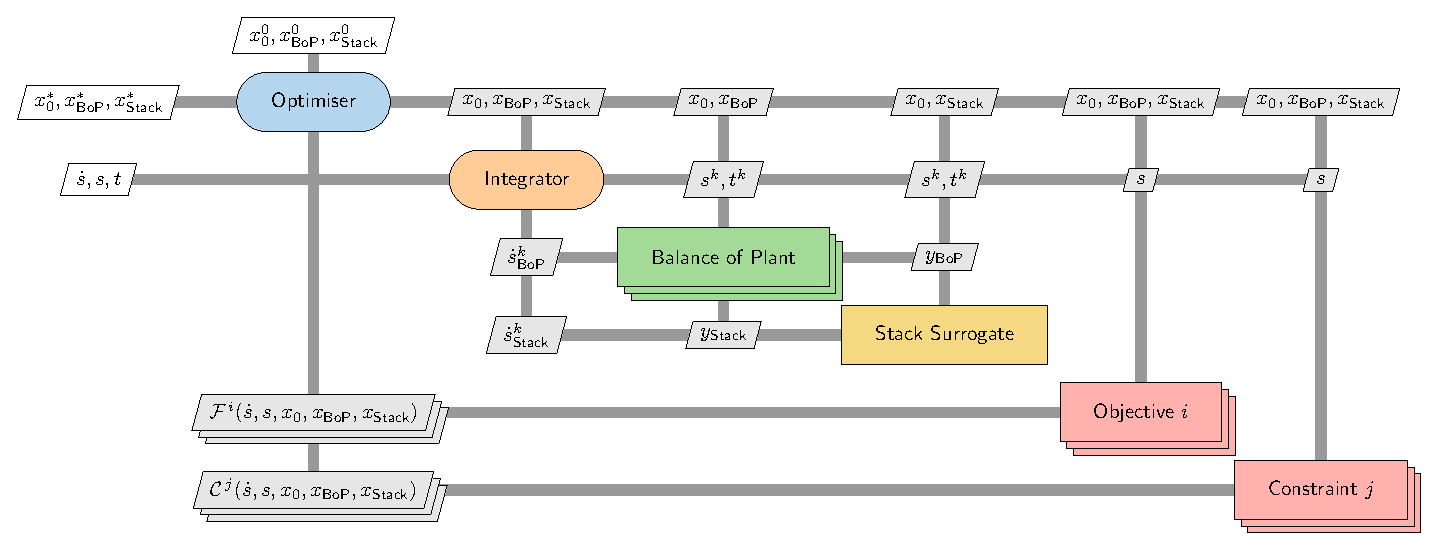
\includegraphics[width=\linewidth]{figures/xdsm.pdf}
		\caption{XDSM Diagram of the proposed fuel cell system model}
		\label{fig:xdsm}
	\end{figure}
\end{center}

